\chapter{Fortbildungen}
\label{cha:fortbildungen}
Die Fortbildungsübersicht zeigt alle zukünftigen Fortbildungen absteigend sortiert nach Datum. Jede Fortbildung wird als Block klar getrennt und übersichtlich dargestellt. In Abbildung \ref{fig:view_training} \textit{\nameref{fig:view_training}} ist eine einzelne Fortbildung exemplarisch abgebildet.

\begin{figure}[h]
 \begin{addmargin}{-0.2\linewidth}
   \centering 
   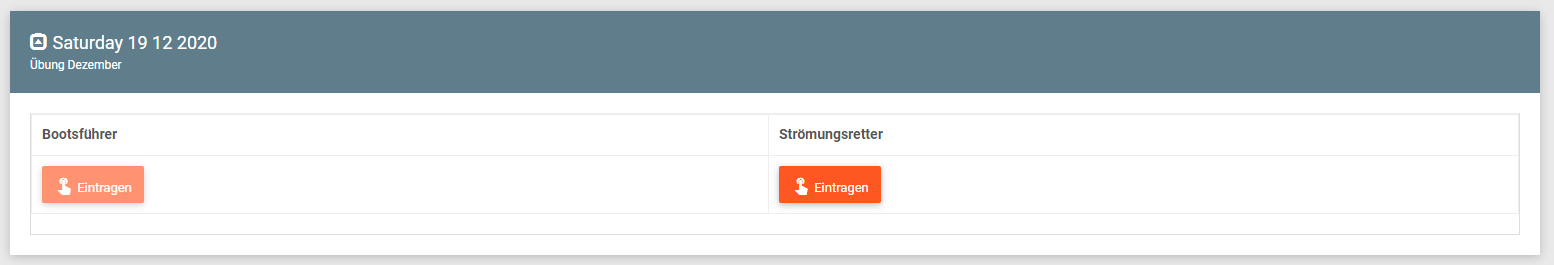
\includegraphics[width=20cm]{Bilder/view_training.png}
 \end{addmargin} 
 \caption[Fortbildungen Übersicht]{DLRG Dienstplan Fortbildung Übersicht}
 \label{fig:view_training}
\end{figure}

\noindent Jede Fortbildung ist mit Tag und Datum beschriftet. Darunter wird der Titel hinterlegt. Die einzelnen Positionen der Fortbildung werden als Tabelle dargestellt. Jeder Position können, wenn die entsprechende Qualifikation vorliegt, beliebig viele Helfer zugewiesen werden.
\noindent Dem Benutzer kann eine Position in drei verschiedenen Ansichten präsentiert werden mit welchen er zum teil Interagieren kann.
Diese sind in der folgenden Tabelle aufgezeigt.

\begin{itemize}
\item Melden: Diese Position ist noch nicht zugeteilt und die entsprechende Qualifikation liegt vor. Der Benutzer kann sich hierzu melden.
\item Melden deaktiviert: Diese Position ist noch nicht zugeteilt. Der Benutzer hat aber nicht die entsprechende Qualifikation und kann sich somit für die Position nicht melden.
\item Meldung zurückziehen: Nach einer Meldung für eine Position kann dies unmittelbar danach wieder zurückgezogen werden.
\end{itemize}

\noindent Positionen können Kommentare beinhalten. Mit Kommentaren werden z.B. auf Besonderheiten zu dieser Position hingewiesen.


\section{Mobile Ansicht}
\label{sec:training_mobile}
Die GUI auf Mobilgeräten, wie \zB Smartphones oder Tablets, weicht von der Desktopversion leicht ab. Die einzelnen Fortbildungen sind eingeklappt und können mit einem Tippen auf den kleinen Pfeil oder das Datum ausgeklappt werden (\ref{fig:view_training_mobile_close} \textit{\nameref{fig:view_training_mobile_close}}). 


\begin{figure}[h]
 \begin{addmargin}{-0.2\linewidth}
   \centering 
   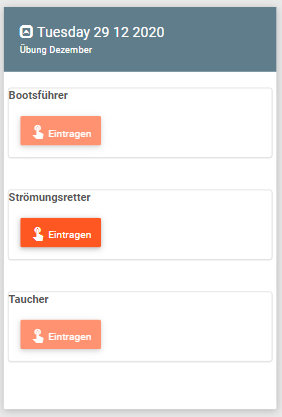
\includegraphics[width=8cm]{Bilder/view_training_mobile.png}
 \end{addmargin} 
 \caption[Fortbildungen Übersicht Mobil]{DLRG Dienstplan Fortbildung Übersicht Mobil}
 \label{fig:view_training_mobile_close}
\end{figure}